\documentclass{standalone}
\usepackage{tikz}
\usetikzlibrary{patterns, positioning}


\begin{document}
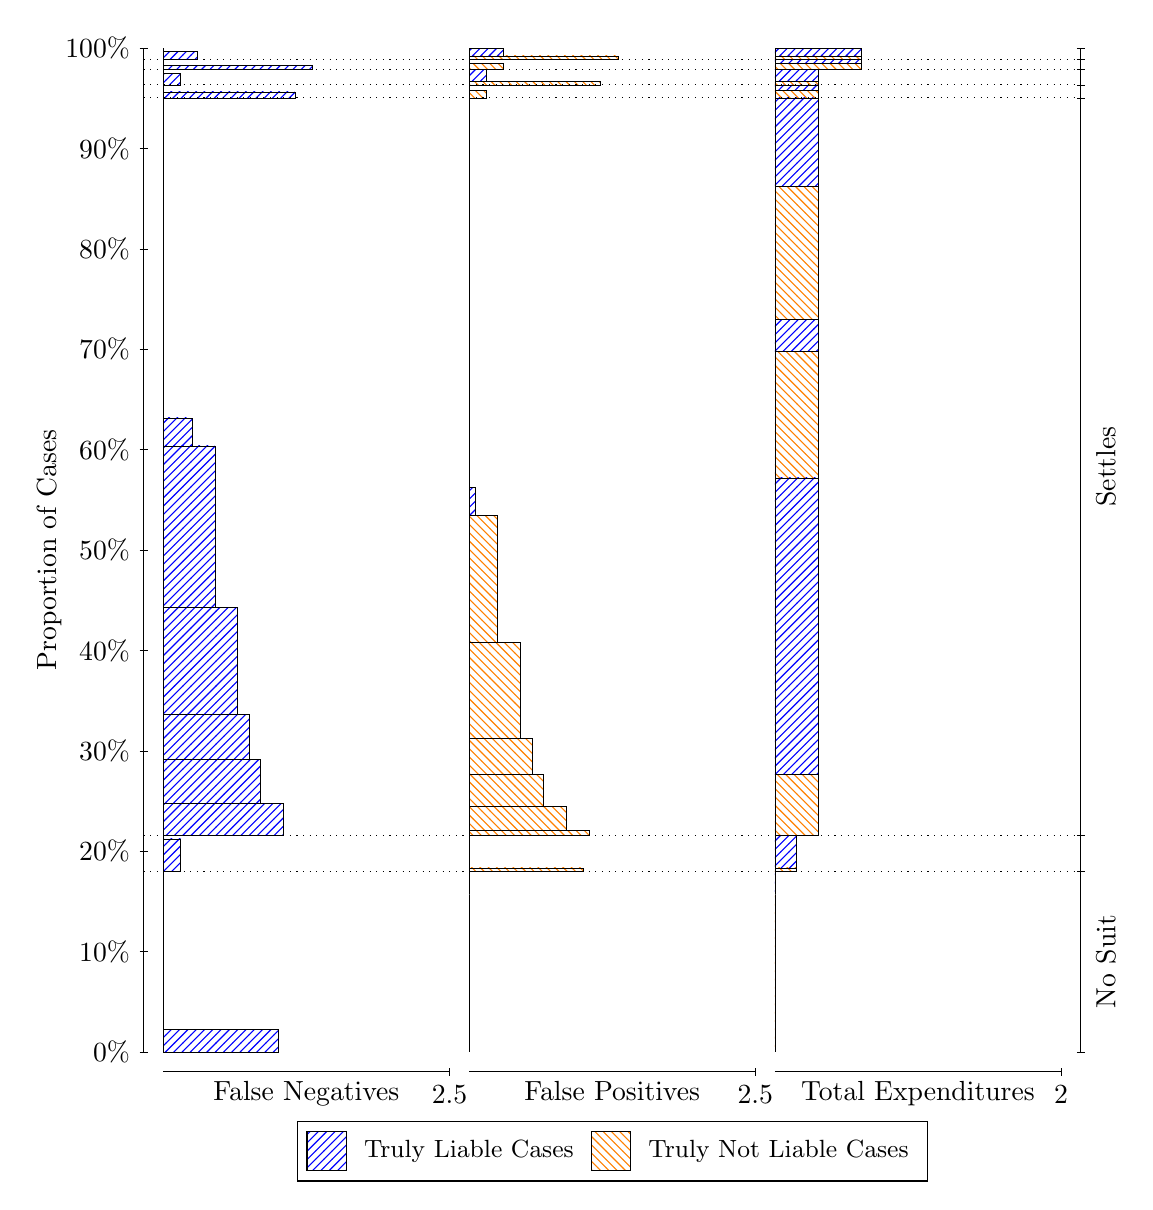
\begin{tikzpicture}
\draw[black, very thin] (1.5,1.75) -- (1.5,14.5);
\node[rotate=90, text=black, anchor=center] at (0.3, 8.125) {Proportion of Cases};
\draw[black, very thin] (1.45,1.75) -- (1.55,1.75);
\node[text=black, anchor=east] at (1.45, 1.75) {0\%};
\draw[black, very thin] (1.45,3.025) -- (1.55,3.025);
\node[text=black, anchor=east] at (1.45, 3.025) {10\%};
\draw[black, very thin] (1.45,4.3) -- (1.55,4.3);
\node[text=black, anchor=east] at (1.45, 4.3) {20\%};
\draw[black, very thin] (1.45,5.575) -- (1.55,5.575);
\node[text=black, anchor=east] at (1.45, 5.575) {30\%};
\draw[black, very thin] (1.45,6.85) -- (1.55,6.85);
\node[text=black, anchor=east] at (1.45, 6.85) {40\%};
\draw[black, very thin] (1.45,8.125) -- (1.55,8.125);
\node[text=black, anchor=east] at (1.45, 8.125) {50\%};
\draw[black, very thin] (1.45,9.4) -- (1.55,9.4);
\node[text=black, anchor=east] at (1.45, 9.4) {60\%};
\draw[black, very thin] (1.45,10.675) -- (1.55,10.675);
\node[text=black, anchor=east] at (1.45, 10.675) {70\%};
\draw[black, very thin] (1.45,11.95) -- (1.55,11.95);
\node[text=black, anchor=east] at (1.45, 11.95) {80\%};
\draw[black, very thin] (1.45,13.225) -- (1.55,13.225);
\node[text=black, anchor=east] at (1.45, 13.225) {90\%};
\draw[black, very thin] (1.45,14.5) -- (1.55,14.5);
\node[text=black, anchor=east] at (1.45, 14.5) {100\%};

\draw[black, very thin] (13.4,1.75) -- (13.4,14.5);
\draw[black, very thin] (13.35,1.75) -- (13.45,1.75);
\node[anchor=west] at (13.35, 1.75) {};
\draw[black, very thin] (13.35,4.0442) -- (13.45,4.0442);
\node[anchor=west] at (13.35, 4.0442) {};
\draw[black, very thin] (13.35,4.5015) -- (13.45,4.5015);
\node[anchor=west] at (13.35, 4.5015) {};
\draw[black, very thin] (13.35,13.868) -- (13.45,13.868);
\node[anchor=west] at (13.35, 13.868) {};
\draw[black, very thin] (13.35,14.033) -- (13.45,14.033);
\node[anchor=west] at (13.35, 14.033) {};
\draw[black, very thin] (13.35,14.228) -- (13.45,14.228);
\node[anchor=west] at (13.35, 14.228) {};
\draw[black, very thin] (13.35,14.352) -- (13.45,14.352);
\node[anchor=west] at (13.35, 14.352) {};
\draw[black, very thin] (13.35,14.5) -- (13.45,14.5);
\node[anchor=west] at (13.35, 14.5) {};

\draw[black, very thin, pattern color=blue, pattern=north east lines] (1.75,1.75) rectangle (3.2033,2.0411);
\draw[black, very thin, pattern color=orange, pattern=north west lines] (1.75,2.0411) rectangle (1.75,4.0442);
\draw[black, very thin, pattern color=blue, pattern=north east lines] (1.75,4.0442) rectangle (1.968,4.4576);
\draw[black, very thin, pattern color=orange, pattern=north west lines] (1.75,4.4576) rectangle (1.75,4.5015);
\draw[black, very thin, pattern color=blue, pattern=north east lines] (1.75,4.5015) rectangle (3.276,4.9079);
\draw[black, very thin, pattern color=blue, pattern=north east lines] (1.75,4.9079) rectangle (2.9853,5.4678);
\draw[black, very thin, pattern color=blue, pattern=north east lines] (1.75,5.4678) rectangle (2.84,6.0372);
\draw[black, very thin, pattern color=blue, pattern=north east lines] (1.75,6.0372) rectangle (2.6947,7.3925);
\draw[black, very thin, pattern color=blue, pattern=north east lines] (1.75,7.3925) rectangle (2.404,9.4462);
\draw[black, very thin, pattern color=blue, pattern=north east lines] (1.75,9.4462) rectangle (2.1133,9.8019);
\draw[black, very thin, pattern color=orange, pattern=north west lines] (1.75,9.8019) rectangle (1.75,13.868);
\draw[black, very thin, pattern color=blue, pattern=north east lines] (1.75,13.868) rectangle (3.4213,13.943);
\draw[black, very thin, pattern color=orange, pattern=north west lines] (1.75,13.943) rectangle (1.75,14.033);
\draw[black, very thin, pattern color=blue, pattern=north east lines] (1.75,14.033) rectangle (1.968,14.18);
\draw[black, very thin, pattern color=orange, pattern=north west lines] (1.75,14.18) rectangle (1.75,14.228);
\draw[black, very thin, pattern color=blue, pattern=north east lines] (1.75,14.228) rectangle (3.6393,14.275);
\draw[black, very thin, pattern color=orange, pattern=north west lines] (1.75,14.275) rectangle (1.75,14.352);
\draw[black, very thin, pattern color=blue, pattern=north east lines] (1.75,14.352) rectangle (2.186,14.453);
\draw[black, very thin, pattern color=orange, pattern=north west lines] (1.75,14.453) rectangle (1.75,14.5);
\draw[black, very thin, pattern color=orange, pattern=north west lines] (5.6333,1.75) rectangle (5.6333,3.7531);
\draw[black, very thin, pattern color=blue, pattern=north east lines] (5.6333,3.7531) rectangle (5.6333,4.0442);
\draw[black, very thin, pattern color=orange, pattern=north west lines] (5.6333,4.0442) rectangle (7.0867,4.0881);
\draw[black, very thin, pattern color=blue, pattern=north east lines] (5.6333,4.0881) rectangle (5.6333,4.5015);
\draw[black, very thin, pattern color=orange, pattern=north west lines] (5.6333,4.5015) rectangle (7.1593,4.5682);
\draw[black, very thin, pattern color=orange, pattern=north west lines] (5.6333,4.5682) rectangle (6.8687,4.8726);
\draw[black, very thin, pattern color=orange, pattern=north west lines] (5.6333,4.8726) rectangle (6.578,5.2759);
\draw[black, very thin, pattern color=orange, pattern=north west lines] (5.6333,5.2759) rectangle (6.4327,5.7359);
\draw[black, very thin, pattern color=orange, pattern=north west lines] (5.6333,5.7359) rectangle (6.2873,6.9566);
\draw[black, very thin, pattern color=orange, pattern=north west lines] (5.6333,6.9566) rectangle (5.9967,8.5679);
\draw[black, very thin, pattern color=blue, pattern=north east lines] (5.6333,8.5679) rectangle (5.706,8.9237);
\draw[black, very thin, pattern color=blue, pattern=north east lines] (5.6333,8.9237) rectangle (5.6333,13.868);
\draw[black, very thin, pattern color=orange, pattern=north west lines] (5.6333,13.868) rectangle (5.8513,13.958);
\draw[black, very thin, pattern color=blue, pattern=north east lines] (5.6333,13.958) rectangle (5.6333,14.033);
\draw[black, very thin, pattern color=orange, pattern=north west lines] (5.6333,14.033) rectangle (7.3047,14.08);
\draw[black, very thin, pattern color=blue, pattern=north east lines] (5.6333,14.08) rectangle (5.8513,14.228);
\draw[black, very thin, pattern color=orange, pattern=north west lines] (5.6333,14.228) rectangle (6.0693,14.305);
\draw[black, very thin, pattern color=blue, pattern=north east lines] (5.6333,14.305) rectangle (5.6333,14.352);
\draw[black, very thin, pattern color=orange, pattern=north west lines] (5.6333,14.352) rectangle (7.5227,14.4);
\draw[black, very thin, pattern color=blue, pattern=north east lines] (5.6333,14.4) rectangle (6.0693,14.5);
\draw[black, very thin, pattern color=orange, pattern=north west lines] (9.5167,1.75) rectangle (9.5167,3.7531);
\draw[black, very thin, pattern color=blue, pattern=north east lines] (9.5167,3.7531) rectangle (9.5167,4.0442);
\draw[black, very thin, pattern color=orange, pattern=north west lines] (9.5167,4.0442) rectangle (9.7892,4.0881);
\draw[black, very thin, pattern color=blue, pattern=north east lines] (9.5167,4.0881) rectangle (9.7892,4.5015);
\draw[black, very thin, pattern color=orange, pattern=north west lines] (9.5167,4.5015) rectangle (10.062,5.2759);
\draw[black, very thin, pattern color=blue, pattern=north east lines] (9.5167,5.2759) rectangle (10.062,9.0407);
\draw[black, very thin, pattern color=orange, pattern=north west lines] (9.5167,9.0407) rectangle (10.062,10.652);
\draw[black, very thin, pattern color=blue, pattern=north east lines] (9.5167,10.652) rectangle (10.062,11.058);
\draw[black, very thin, pattern color=orange, pattern=north west lines] (9.5167,11.058) rectangle (10.062,12.739);
\draw[black, very thin, pattern color=blue, pattern=north east lines] (9.5167,12.739) rectangle (10.062,13.868);
\draw[black, very thin, pattern color=orange, pattern=north west lines] (9.5167,13.868) rectangle (10.062,13.958);
\draw[black, very thin, pattern color=blue, pattern=north east lines] (9.5167,13.958) rectangle (10.062,14.033);
\draw[black, very thin, pattern color=orange, pattern=north west lines] (9.5167,14.033) rectangle (10.062,14.08);
\draw[black, very thin, pattern color=blue, pattern=north east lines] (9.5167,14.08) rectangle (10.062,14.228);
\draw[black, very thin, pattern color=orange, pattern=north west lines] (9.5167,14.228) rectangle (10.607,14.305);
\draw[black, very thin, pattern color=blue, pattern=north east lines] (9.5167,14.305) rectangle (10.607,14.352);
\draw[black, very thin, pattern color=orange, pattern=north west lines] (9.5167,14.352) rectangle (10.607,14.4);
\draw[black, very thin, pattern color=blue, pattern=north east lines] (9.5167,14.4) rectangle (10.607,14.5);
\draw[black, dotted] (1.5,4.0442) -- (13.4,4.0442);
\draw[black, dotted] (1.5,4.5015) -- (13.4,4.5015);
\draw[black, dotted] (1.5,13.868) -- (13.4,13.868);
\draw[black, dotted] (1.5,14.033) -- (13.4,14.033);
\draw[black, dotted] (1.5,14.228) -- (13.4,14.228);
\draw[black, dotted] (1.5,14.352) -- (13.4,14.352);
\draw[black, very thin] (1.75,1.5) -- (5.3833,1.5);
\node[text=black, anchor=north] at (3.5667, 1.5) {False Negatives};
\draw[black, very thin] (5.3833,1.45) -- (5.3833,1.55);
\node[text=black, anchor=north] at (5.3833, 1.45) {2.5};

\draw[black, very thin] (5.6333,1.5) -- (9.2667,1.5);
\node[text=black, anchor=north] at (7.45, 1.5) {False Positives};
\draw[black, very thin] (9.2667,1.45) -- (9.2667,1.55);
\node[text=black, anchor=north] at (9.2667, 1.45) {2.5};

\draw[black, very thin] (9.5167,1.5) -- (13.15,1.5);
\node[text=black, anchor=north] at (11.333, 1.5) {Total Expenditures};
\draw[black, very thin] (13.15,1.45) -- (13.15,1.55);
\node[text=black, anchor=north] at (13.15, 1.45) {2};

\node[text=black, centered, rotate=90] at (13.72, 2.8971) {No Suit};

\node[text=black, centered, rotate=90] at (13.72, 9.1849) {Settles};





\draw (7.449999999999999,1.5) node[draw=none] (baseCoordinate) {};
\begin{scope}[align=center]
        \matrix[scale=0.5, draw=black, below=0.5cm of baseCoordinate, nodes={draw}, column sep=0.1cm]{
            \node[rectangle, draw, minimum width=0.5cm, minimum height=0.5cm, pattern color=blue, pattern=north east lines] {}; &
            \node[draw=none, font=\small, text=black] (B) {Truly Liable Cases}; &
            \node[rectangle, draw, minimum width=0.5cm, minimum height=0.5cm, pattern color=orange, pattern=north west lines] {}; &
            \node[draw=none, font=\small, text=black] (B) {Truly Not Liable Cases}; \\
            };
\end{scope}

\end{tikzpicture}
\end{document}